\documentclass[12pt]{article}
\usepackage{indentfirst}
\usepackage{enumitem}
\usepackage{amsmath}
\usepackage{multicol}
\setlength{\jot}{2ex}
\usepackage{mathrsfs}
\usepackage{graphicx}
\usepackage{wrapfig}
\usepackage{booktabs}
\usepackage[letterpaper, margin=1in]{geometry}
\usepackage{fancyhdr}
\pagestyle{fancy}
\fancyhead[R]{Homework 1}
\fancyfoot[C]{\thepage}
\renewcommand{\headrulewidth}{1pt}
\renewcommand{\footrulewidth}{1pt}
\usepackage [autostyle, english = american]{csquotes}
\MakeOuterQuote{"}
\renewcommand{\baselinestretch}{1.0}
\newcommand{\objects}[2]{%
  \leavevmode\vbox{\hbox{#1}\nointerlineskip\hbox{#2}}%
}
\begin{document}
    \section*{Problem 7.3}
    \begin{figure}[h]
        \centering
        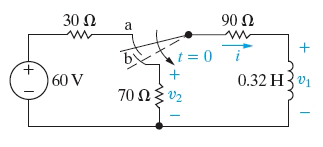
\includegraphics[width=0.5\textwidth]{7.3 Figure.png}
    \end{figure}
    \par In the circuit shown above, the switch makes contact with position $b$ just before breaking contact with position $a$. As already mentioned, this is known as a make-before-break switch and is designed so that the switch does not interrupt the current in an inductive circuit. The interval of time between "making" and "breaking" is assumed to be negligible. The switch has been in the $a$ position for a long time. At $t = 0$ the switch is thrown from position $a$ to position $b$.
    \subsubsection*{Part A} Determine the initial current in the inductor: \\
    \par Since the switch has been at position $a$ for a long time and the steady state behavior of an inductor is equal to a short circuit, the current can be calculated using Ohm's Law with the two resistors that are in series.
    \[
        i(0) = \frac{V_s}{R_{eq}} = \frac{60}{30 + 90} = \boxed{0.5 A}
    \]
    \subsubsection*{Part B} Determine the time constant for $t > 0$: \\
    \par At time $t = 0$, the switch is moved to position $b$ and the inductor begins to discharge. The source and the $30\ \Omega$ resistors can be ignored leaving just the RL circuit. The time constant for an RL circuit is equal to
    $\frac{L}{R}$.
    \[
        \tau = \frac{L}{R} = \frac{0.32}{90+70} = \boxed{0.002\ s}
    \]
    \subsubsection*{Part C} Select the correct expression for $i(t)$ for $t > 0$: \\
    \par The expression for $i(t)$ for an RL circuit takes the form, $I_0e^{-\frac{R}{L}t}$, where $I_0$ is the initial value of the current in the inductor and the $\frac{R}{L}$ is the inverse $\tau$, $\frac{1}{\tau}$. Using this as well, the expression can also be written as, $I_0e^{-\frac{t}{\tau}}$. Plugging into this expression yields an expression for the current as a function of time,
    \[
        \boxed{i(t) = 0.5e^{-500t}}
    \]
    \subsubsection*{Part D} Select the correct expression for $v_1(t)$ for $t > 0$: \\
    \par Since $v(t)$ is equal to $L\frac{di}{dt}$, the expression for the voltage can be given as,
    \[
        (0.32) \frac{d}{dt} \left( 0.5e^{-500t} \right) =
        (0.32)(0.5)(-500)e^{-500t} = \boxed{-80e^{-500t}}
    \]
    \subsubsection*{Part E} Select the correct expression for $v_2(t)$ for $t > 0$: \\
    \par Since $v_2$ is across a resistor, we can use Ohm's Law and multiply the resistance and the current to get the voltage across the resistor,
    \[
        (70)(0.5e^{-500t}) = \boxed{35e^{-500t}}
    \]
    \subsubsection*{Part F} What percentage of the initial energy stored in the inductor is dissipated in the $90\ \Omega$ resistor $3\ ms$ after the switch is thrown from position $a$ to position $b$? \\
    \par The initial energy of the resistor can be given by the expression,
    \[
        w_{i} = \frac{1}{2} L I_0^2
    \]
    and the final energy can be given by integrating the power from the initial time to 3 $ms$,
    \[
        w_{f} = \int_0^{0.003} \left( 0.5e^{-500t} \right)^2 (90)\ dt.
    \]
    Finding the initial energy we get,
    \[
        w_i = \frac{1}{2} (0.32) (0.5)^2 = 0.04\ J
    \]
    and solving for the final energy across the 90 $\Omega$ resistor,
    \[
        w_f = 0.0214\ J.
    \]
    Finding the percentage dissipated would be,
    \[
        \frac{0.0214}{0.04} \times 100 = \boxed{53.45\%}
    \]
    \newpage
    \section*{Problem 7.7}
    \begin{figure}[h]
        \centering
        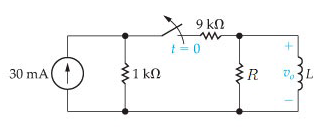
\includegraphics[width=0.5\textwidth]{7.7 Figure.png}
    \end{figure}
    \par In the circuit the switch has been closed for a long time before opening at time $t = 0$.
    \subsubsection*{Part A} Find the value of $L$ so that $v_0(t)$ equals $0.5v_0(0^{+})$ when $t = 1.6\ ms$. Take $R = 13\ \Omega$. \\
    \par Before opening the switch, in essence the circuit is equal to a current source in series with a 9 $k\Omega$ resistor since at a steady state inductors act like short circuits. This means that initially, the voltage across the inductor is equal to $IR$ by Ohm's Law. This gives the value of $v_0(0)$ to be $(9000)(0.03) = 270 V$.
    \par Now for the natural response circuit after the switch is opened, we get voltage as a function of time which is defined as taking the form,
    \[
        v_0(t) = V_0e^{-Rt / L}.
    \]
    Plugging in the values for $V_0$ and $R$, and evaluating for time $t = 1.6\ ms$,
    \[
        v_0(0.0016) = 270e^{-(13)(0.0016) / L} = 270e^{-0.0208 / L}.
    \]
    Now to find the value of $L$ that makes the equation $v_0(0.0016) = 0.5v_0(0)$ true we would plug the expressions into the equation and solve for $L$.
    \begin{align*}
        (0.5)(270) &= 270e^{-0.0208 / L} \\
        0.5 &= e^{-0.0208 / L} \\
        \ln(0.5) &= -0.0208 / L \\
        L &= \frac{-0.0208}{\ln(0.5)} \\
        L &= \boxed{30.01\ mH}
    \end{align*}
    \subsubsection*{Part B} Find the percentage of the stored energy that has been dissipated in the resistor $R$ when $t = 1.6\ ms$. \\
    \par The expression for the current as a function of time can be given as,
    \[
        i(t) = I_0e^{-Rt / L} = 0.03e^{-13t / 0.03} = 0.03e^{-433.33t}.
    \]
    The initial energy can be given by the expression $\frac{1}{2} L I_0^2$, where $I_0$ is the initial current in the inductor.
    \[
        w_i = \frac{1}{2} (0.03) (0.03)^2 = 1.35 \times 10^{-5}\ J.
    \]
    The final energy can be given by integrating the power $i^2R$,
    \[
        w_f = \int_0^{0.0016} (13) (0.03e^{-13t / 0.03})^2\ dt = 1.0126 \times 10^{-5}\ J.
    \]
    Finally finding the percentage,
    \[
        \frac{1.0126 \times 10^{-5}}{1.35 \times 10^{-5}} \times 100 =
        \boxed{75.009\%}
    \]
    \section*{Problem 7.12}
    \begin{figure}[h]
        \centering
        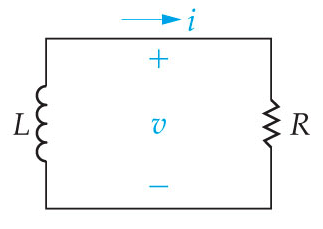
\includegraphics[width=0.3\textwidth]{7.12 Figure.png}
    \end{figure}
    \par In the circuit the voltage and current expressions are, $v(t) = 240e^{-15t}$ and $i(t) = 5.1e^{-15t}$ for $t > 0$.
    \subsubsection*{Part A} Find $R$. \\
    \par Using Ohm's Law, $R = \frac{V}{I}$,
    \[
        R = \frac{240e^{-15t}}{5.1e^{-15t}} = \frac{240}{5.1} = \boxed{47.059\ \Omega}
    \]
    \subsubsection*{Part B} Find $L$. \\
    \par Since $v = L \frac{di}{dt}$,
    \[
        L = \frac{240e^{-15t}}{\frac{d}{dt}\left( 5.1e^{-15t} \right) } =
        \frac{240e^{-15t}}{5.1(-15e^{-15t})} = \boxed{3.1373\ H}
    \]
    \subsubsection*{Part C} Find $\tau$. \\
    \par Since $\tau = \frac{L}{R}$,
    \[
        \tau = \frac{3.1373}{47.059} = \boxed{66.7\ ms}
    \]
    \subsubsection*{Part D} Find the initial energy stored in the inductor. \\
    \par Since $w = \frac{1}{2} L i^2$,
    \[
        w_i = \frac{1}{2} (3.1373) (5.1)^2 = \boxed{40.8\ J}
    \]
    \subsubsection*{Part E} Find the time in milliseconds it takes to dissipate 60\% of the initial stored energy. \\
    \par Since \% dissipated = $w_f / w_i \times 100$,
    \begin{align*}
        .60 &= w_f / 40.8 \\
        w_f &= 24.48\ J
    \end{align*}
    and since $w_f$ is the integral of the power $i^2R$,
    \begin{align*}
        24.48 &= \int_0^{t} (5.1e^{-15t})^2 (47.059)\ dt \\
        24.48 &= (47.059) (5.1)^2 \int_0^{t} e^{-30t}\ dt
    \end{align*}
    solving the integral and then for $t$,
    \begin{align*}
        \frac{24.48}{(47.059) (5.1)^2} &= -\frac{1}{30}(e^{-30t}-1) \\
        (0.02) (-30) &= e^{-30t} - 1 \\
        -0.6 &= e^{-30t} - 1 \\
        0.4 &= e^{-30t} \\
        \ln(0.4) &= -30t \\
        t = \frac{\ln(0.4)}{-30} &= \boxed{30.5\ ms}
    \end{align*}
    \newpage
    \section*{Problem 7.21}
    \begin{figure}[h]
        \centering
        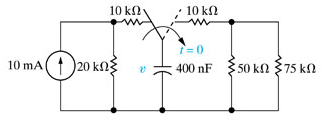
\includegraphics[width=0.5\textwidth]{7.21 Figure.png}
    \end{figure}
    \par The switch in the circuit has been in the left position for a long time. At $t = 0$ it moves to the right position and stays there.
    \subsubsection*{Part A} Find the initial voltage drop across the capacitor. \\
    \par In steady state, capacitors act as an open circuit, so the voltage across the capacitor would be the same as the voltage across the 20 $k\Omega$ resistor and this is given by,
    \[
        V = IR = (0.01) (20000) = \boxed{200\ V}
    \]
    \subsubsection*{Part B} Find the initial energy stored by the capacitor. \\
    \par The energy stored in a capacitor is given by $w = \frac{1}{2} C V^2$,
    \[
        w = \frac{1}{2} (400 \times 10^{-9}) (200)^2 = \boxed{8\ mJ}
    \]
    \subsubsection*{Part C} Find the time constant of the circuit. \\ \par $\tau$ for an RC circuit is equal to $RC$. The $R$ will be the equivalent resistance for the right side, and $C$ will be the capacitance,
    \[
        R = \left( (75)^{-1} + (50)^{-1} \right)^{-1} + 10 = 40\ k\Omega
    \]
    \[
        \tau = (40 \times 10^{3}) (400 \times 10^{-9}) = \boxed{16\ ms}
    \]
    \subsubsection*{Part D} Write the expression for the capacitor voltage $v(t)$. \\
    \par The expression for voltage as a function of time for an RC circuit takes the form $V_0e^{-t / RC}$,
    \[
        v(t) = 200e^{-\frac{t}{0.016}} = \boxed{200e^{-62.5t}}
    \]
    \section*{Problem 7.26}
    \begin{figure}[h]
        \centering
        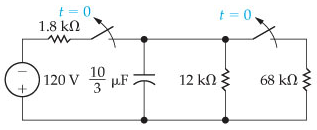
\includegraphics[width=0.5\textwidth]{7.26 Figure.png}
    \end{figure}
    \par In the circuit shown in the figure, both switches operate together; that is, they either open or close at the same time. The switches are closed a long time before opening at $ t = 0 $.
    \subsubsection*{Part A} How many microjoules of energy have been dissipated in the $ 12\ k\Omega $ resistor $ 16\ ms $ after the switches open? \\
    \par To find the energy dissipated we must first find the expression for voltage across the capacitor.
    \[
        v_c(t) = V_0 e^{-t / RC}
    \]
    \begin{align*}
        V_0 &= -120 \left( \frac{(12)(68) / (12+68)}{1.8 + (12)(68) / (12+68)} * 10^{3} \right) \\
        V_0 &= -102\ V
    \end{align*}
    \[
        \frac{1}{\tau} = ((12 * 10^{3})(\frac{10}{3} * 10^{-6}))^{-1} = 25
    \]
    \[
        v_c (t) = -102 e^{-25t}
    \]
    Now that we have the equation for the voltage across the capacitor, we can find the energy dissipated,
    \begin{align*}
        \omega_{diss} &= \int_0^{16*10^{-3}} \frac{(-102 e^{-25t})^2 }{12 * 10^{3}}\ dt \\
        \omega_{diss} &= 0.009549\ J = \boxed{9550\ \mu J}
    \end{align*}
    \subsubsection*{Part B} How long does it take to dissipate 62 \% of the initially stored energy? \\
    \par Finding the initial energy in the capacitor,
    \[
        \omega_{i} = \frac{1}{2} \left( \frac{10}{3} * 10^{-6} \right) (-102)^2 = 17.34\ mJ
    \]
    and since,
    \[
        0.62 = \frac{\omega_{f}}{\omega_{i}}
    \]
    \[
        \omega_{f} = (0.62) (0.01734) = 10.751\ mJ
    \]
    This value can be set to the integral for the energy,
    \[
        \int_0^t \frac{(-102e^{-25t})^2}{12 * 10^{3}}\ dt = 10.751 * 10^{-3}
    \]
    and solving this integral for $ t $ will give us the value we are looking for.
    \[
        \int_0^t e^{-50t}\ dt  = \frac{(10.751 * 10^{3})(12 * 10^{3})}{102^2}
    \]
    \[
        0.0124 = -\frac{1}{50} \left( e^{-50t} - 1 \right)
    \]
    \[
        ((0.0124)(-50)) + 1 = e^{-50t}
    \]
    \[
        \ln(0.38) = -50t
    \]
    \[
        t = \frac{\ln(0.38)}{-50} = \boxed{19.4\ ms}
    \]
    \section*{Problem 7.35}
    \begin{figure}[h]
        \centering
        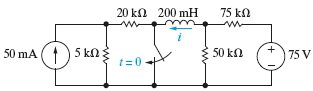
\includegraphics[width=0.6\textwidth]{7.35 Figure.png}
    \end{figure}
    \par After the switch in the circuit has been open for a long time, it is closed at $ t = 0 $.
    \subsubsection*{Part A} Calculate the initial value of $ i $. \\
    \par First simplify the circuit to a resistor network and convert the current source to a voltage source. Using that we can write a node equation for which we solve for the voltage, and the current through the $ 20\ k\Omega $ resistor which is equal to the initial current through the inductor.
    \[
        \frac{v_0 - 250}{25 * 10^{3}} + \frac{v_0}{50 * 10^{3}} + \frac{v_0 - 75}{75 * 10^{3}} = 0
    \]
    \[
        v_0 = 150\ V
    \]
    Using this, the value of the current would be,
    \[
        i_{20} = \frac{v_0 - 250}{25 * 10^{3}} = -0.004\ A = \boxed{-4\ mA}
    \]
    \subsubsection*{Part B} Calculate the final value of $ i $. \\
    \par The final current of an inductor resembles the current of the source and in this case, after a long time with the switch closed, the current in the inductor will be equal to the current across the $ 75\ k\Omega $ resistor.
    \[
        i_{75} = \frac{75\ V}{75 * 10^{3}\ \Omega} = \boxed{1\ mA}
    \]
    \subsubsection*{Part C} Find the value of $ i(t) $ when $ t \ge 0 $. \\
    \par The current as a function of time will take the form,
    \[
        i(t) = i(\infty) + (i(t_0) - i(\infty)) e^{-(t - t_0) / \tau}
    \]
    and plugging in the known values into this equation we get,
    \[
        i(t) = (1) + ((-4) - (1)) e^{(-30 * 10^{3}) t / (200 * 10 ^{-3})}
    \]
    \[
        \boxed{i(t) = 1 - 5 e^{-150000t}\ mA}
    \]
    \section*{Problem 7.51}
    \begin{figure}[h]
        \centering
        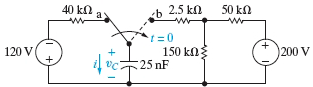
\includegraphics[width=0.6\textwidth]{7.51 Figure.png}
    \end{figure}
    \par Assume that the switch in the circuit has been in position $ a $ for a long time and that at $ t = 0 $ it is moved to position $ b $.
    \subsubsection*{Part A} Find $ v_c (0^+) $. \\
    \par At steady state, the voltage across the capacitor will be equal to the source voltage connected across it.
    \[
        v_c (0^+) = \boxed{-120\ V}
    \]
    \subsubsection*{Part B} Find $ v_c (\infty) $. \\
    \par This time, the steady state will be achieved with the switch in position $ b $. Using voltage division we get,
    \[
        v_c (\infty) = 200 * \left( \frac{150}{200} \right) = \boxed{150\ V}
    \]
    \subsubsection*{Part C} Find $ \tau $ for $ t > 0 $. \\
    \par Using source transformation to find the equivalent resistance and the voltage we get a voltage source of $ 150\ V $ with a resistor of $ 40\ k\Omega $, in series with the capacitor. The time constant therefore would be,
    \[
        \tau = RC = (40 * 10^{3})(25 * 10^{-9}) = \boxed{1\ ms}
    \]
    \subsubsection*{Part D} Find $ i(0^+) $. \\
    \par Using the circuit formed in the previous part we can find the current as the current as,
    \[
        i(0^+) = \frac{V_s - v_c}{R_{eq}}
    \]
    since the capacitor initially is at a voltage of $ -120\ V $. This must be factored in since the capacitor has a voltage across it when the switch is thrown from position $ a $ to position $ b $.
    \[
        i(0^+) = \frac{(150) - (-120)}{40 * 10^{3}} = \boxed{6.75\ mA}
    \]
    \subsubsection*{Part E} Find the expression for $ v_c(t) $ for $ t > 0 $. \\
    \par In order to write this we can follow the general form for the voltage or current in an RC circuit,
    \[
        v(t) = v(\infty) + (v(t_0) - v(\infty)) e^{-(t - t_0) / \tau}
    \]
    Plugging in to this we get,
    \begin{align*}
        v_c(t) &= 150 + (-120 - 150) e^{-t / 0.001} \\
        v_c(t) &= \boxed{150 - 270 e^{-1000t}\ V}
    \end{align*}
    \newpage
    \section*{Problem 7.78}
    \begin{figure}[h]
        \centering
        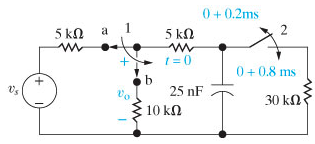
\includegraphics[width=0.5\textwidth]{7.78 Figure.png}
    \end{figure}
    \par In the circuit, switch 1 has been in position $ a $ and switch 2 has been closed for a long time. At $ t =  0 $, switch 1 moves instantaneously to position $ b $. $ 200\ \mu s $ later, switch 2 opens, remains open for $ 600\ \mu s $, and then closes again.
    \subsubsection*{Part A} Find $ v_{o}\ 1\ ms $ after switch 1 makes contact with terminal $ b $ if $ v_{s} = 15\ V $. \\
    \par Initially, the voltage across the capacitor will be equal to the voltage across the $ 30\ k\Omega $ resistor. This can be found using voltage division and treating the capacitor branch as an open circuit.
    \[
        v_c = \frac{30}{40} * 15 = 11.25\ V
    \]
    Now, we must look at the configuration between $ t = 0 $ and $ t = 200\ \mu s $ before switch 2 is opened. This leaves the capacitor in parallel with the series combination of 5 and 10 $ k\Omega $ and the $ 30\ k\Omega $ resistors. and the configuration will follow the natural response of an RC circuit. The initial voltage is the 11.25 $ V $ calculated in the previous step, and $ \tau $ will be given by $ ((15 * 10^{3})\ ||\ (30 * 10^{3}))(25 * 10^{-9}) $.
    \[
        v_c(t) = 11.25 e^{-4000t}
    \]
    The circuit is in this configuration for $ 200\ \mu s $ so the voltage just before switch 2 is opened can be given by,
    \[
        v_c(200 * 10^{-6}) = 11.25 e^{-4000(200 * 10^{-6})} = 5.055\ V
    \]
    When switch 2 is opened, the circuit is simply the capacitor in series with the 5 and the 10 $ k\Omega $ resistors. Using the value at $ t = 200\ \mu s $ as the initial value and $ \tau $ as $ (15 * 10^{3})(25 * 10^{-9}) $, we can write the equation for the voltage of the capacitor as,
    \[
        v_c(t) = 5.055 e^{-t / 3.75 * 10^{-4}}
    \]
    Since the circuit is in this configuration from $ 200\ \mu s < t < 800\ \mu s $ when switch 2 is reclosed, the initial voltage for the next configuration can be given by,
    \[
        v_c(600 * 10^{-6}) = 5.055 e^{-(600 * 10^{-6}) / 3.75 * 10^{-4}} = 1.021\ V
    \]
    Finally, the last configuration is the same as the one from 0 to $ 200\ \mu s $, and using the final voltage of the last configuration as the initial voltage of this one we get the equation,
    \[
        v_c(t) = 1.021 e^{-4000t}
    \]
    Using this equation and the fact that the circuit is in this configuration for $ 200\ \mu s $, we can find the voltage across the capacitor, $ v_c $, after $ 1\ ms $.
    \[
        v_c(200 * 10^{-6}) = 1.021 e^{-4000(200 * 10^{-6})} = 0.4586\ V
    \]
    Lastly, we can find the voltage across the $ 10\ k\Omega $ resistor, $ v_{o} $, using voltage division.
    \[
        v_{o} = 0.4586\left( \frac{10}{15} \right) = \boxed{0.306\ V}
    \]
\end{document}
